% In this section, the layer is described in some detail in terms of its specific subsystems. Describe each of the layers and its subsystems in a separate chapter/major subsection of this document. The content of each subsystem description should be similar. Include in this section any special considerations and/or trade-offs considered for the approach you have chosen.
This will be the actual server or the back end for the application which will handle most of the heavy computations required for the application. The back end will handle requests coming in from the front end, interact with the database and the data control layer to provide the front end with the appropriate response. The back end contains the following subsystems:

\begin{figure}[h!]
	\centering
 	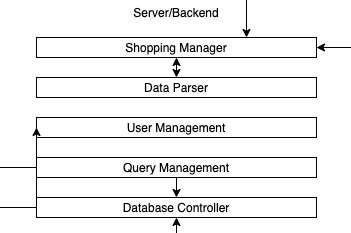
\includegraphics[width=0.60\textwidth]{images/Server.png}
 \caption{Back End Subsystems}
\end{figure}

\subsection{Shopping Manager Subsystem}
The shopping manager subsystem will deal with all the shopping related computation. It will get requests directly from the shopping subsystem of the front end. Then it will get the required shopping data from the Data Controller layer, use the Data parser subsystem to parse the data into standard format, and then send it as a response to the front-end.

% \begin{figure}[h!]
% 	\centering
%  	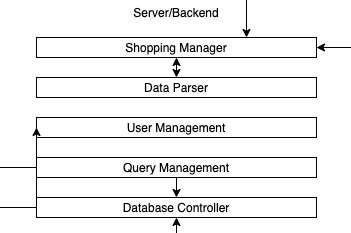
\includegraphics[width=0.60\textwidth]{images/Server.png}
%  \caption{Example subsystem description diagram}
% \end{figure}

\subsubsection{Assumptions}
The requests from the front end are in standard format and the data is found by the data controller layer.

\subsubsection{Responsibilities}
% Each of the responsibilities/features/functions/services of the subsystem as identified in the architectural summary must be expanded to more detailed responsibilities. These responsibilities form the basis for the identification of the finer-grained responsibilities of the layer's internal subsystems. Clearly describe what each subsystem does.
The shopping manager subsystem is responsible for getting prices for grocery items, entire shopping lists, and calculating the optimal route for shopping based on user preferences such as brand and maximum travel distance. The algorithm will optimize by distance and price to generate the list of items and where to buy them for the user and send this data back to the front end.

\subsubsection{Subsystem Interfaces}

\begin {table}[H]
\caption {Subsystem interfaces} 
\begin{center}
    \begin{tabular}{ | p{1cm} | p{6cm} | p{3cm} | p{3cm} |}
    \hline
    ID & Description & Inputs & Outputs \\ \hline
    \#1 & Request for a single item & \pbox{3cm}{Standard name \\ for that item} & \pbox{3cm}{List of places and prices}  \\ \hline
    \#2 & Optimal route & \pbox{3cm}{Grocery List} & \pbox{3cm}{Optimal Route}  \\ \hline
    \#3 & data from controller & \pbox{3cm}{Take data from controller} & \pbox{3cm}{Send it to parser}  \\ \hline
    \end{tabular}
\end{center}
\end{table}

\subsection{User Management Subsystem}
The user management subsystem will handle all requests from the front end related to the user of the application and give back appropriate response. It will keep track of the currently logged in user.

\subsubsection{Assumptions}
There are no assumptions for this subsystem.

\subsubsection{Responsibilities}
% Each of the responsibilities/features/functions/services of the subsystem as identified in the architectural summary must be expanded to more detailed responsibilities. These responsibilities form the basis for the identification of the finer-grained responsibilities of the layer's internal subsystems. Clearly describe what each subsystem does.
The user management subsystem will be responsible for handling all user related tasks such as updating user profile and keeping track of their preferences. This will also keep track of how long the user has been logged in and determine when to automatically log them out.

\subsubsection{Subsystem Interfaces}

\begin {table}[H]
\caption {Subsystem interfaces} 
\begin{center}
    \begin{tabular}{ | p{1cm} | p{5cm} | p{5cm} | p{5cm} |}
    \hline
    ID & Description & Inputs & Outputs \\ \hline
    \#1 & Login & \pbox{5cm}{Response from Query Manager} & \pbox{5cm}{Keep track of the logged in user}  \\ \hline
    \#2 & Update user profile & \pbox{5cm}{New user data} & \pbox{5cm}{Success or failure}  \\ \hline
    \end{tabular}
\end{center}
\end{table}

\subsection{Query Management Subsystem}
The query management subsystem will handle all requests from the front end that needs a result from a query on the database and give back the appropriate response. Also give the current logged in users info to user management subsystem to keep track of the user. 

\subsubsection{Assumptions}
Email format is checked at the front end before passing it to the Query Management System.

\subsubsection{Responsibilities}
% Each of the responsibilities/features/functions/services of the subsystem as identified in the architectural summary must be expanded to more detailed responsibilities. These responsibilities form the basis for the identification of the finer-grained responsibilities of the layer's internal subsystems. Clearly describe what each subsystem does.
The query management subsystem will be responsible for handling all user related tasks such as account creation, logging in, and logging out. For user registration it would take username or email, password and other user details and store it into the database. For login it would take the username or email, \& password and check it against the username stored in the database and determine login success and relay the message back to the front end and also get the user data and pass it to user management to keep track of the logged in user.

The query management subsystem will also create all queries for users when they want to view their shopping lists, meal plans, and recipes. It will also create queries for users when they are searching for grocery items to add to their shopping lists.

\subsubsection{Subsystem Interfaces}

\begin {table}[H]
\caption {Subsystem interfaces} 
\begin{center}
    \begin{tabular}{ | p{1cm} | p{5cm} | p{5cm} | p{5cm} |}
    \hline
    ID & Description & Inputs & Outputs \\ \hline
    \#1 & Register & \pbox{5cm}{Email and password} & \pbox{5cm}{Response from database}  \\ \hline
    \#2 & Login & \pbox{5cm}{Email and password} & \pbox{5cm}{Success or Failure}  \\ \hline
    \#3 & Requests from Shopping List & \pbox{5cm}{Username or Email} & \pbox{5cm}{User's Shopping List from Database}  \\ \hline
    \#4 & Requests from Recipes & \pbox{5cm}{Username or Email} & \pbox{5cm}{User's stored recipes}  \\ \hline
    \#5 & Search for Grocery Items & \pbox{5cm}{Search text from front-end} & \pbox{5cm}{Search Results}  \\ \hline
    \end{tabular}
\end{center}
\end{table}

\subsection{Database Controller Subsystem}
The database controller will handle all the communication of the application to the database. It will give responses to the query management system with the required data extracted from the database.

\subsubsection{Assumptions}
The query management system will protect the database controller from attacks like SQL Injection.

\subsubsection{Responsibilities}
% Each of the responsibilities/features/functions/services of the subsystem as identified in the architectural summary must be expanded to more detailed responsibilities. These responsibilities form the basis for the identification of the finer-grained responsibilities of the layer's internal subsystems. Clearly describe what each subsystem does.
The database controller subsystem will be responsible for handling all communications to and from the database. It will create the initial connection with the database on the application startup. Every query to the database will go through this controller. It will get login, registration, shopping list, meal plans, recipes, grocery items, and update queries from the query management system and provide responses from the database.

\subsubsection{Subsystem Interfaces}

\begin {table}[H]
\caption {Subsystem interfaces} 
\begin{center}
    \begin{tabular}{ | p{1cm} | p{5cm} | p{5cm} | p{5cm} |}
    \hline
    ID & Description & Inputs & Outputs \\ \hline
    \#1 & Requests from Query manager & \pbox{5cm}{Email and password} & \pbox{5cm}{Response from database}  \\ \hline
    \end{tabular}
\end{center}
\end{table}

